\subsubsection{1.5. Kiến trúc Decoupled GNN-ML}

\indent\indent Đề tài thực hiện thực nghiêm trên các kiến trúc mô hình \textit{Decoupled GNN-ML}. Lựa chọn này xuất phát từ việc nhận diện các giới hạn của các lớp nơ-ron trong mạng đồ thị thuần túy. Các sự kết hợp này giải quyết hạn chế thiết lập các ranh giới rõ ràng trên dữ liệu không đồng nhất của các lớp nơ-ron trong mạng đồ thị bằng cách tách rời quy trình học đặc trưng và quy trình quyết định. Sơ đồ luồng xử lý được mô tả tại \textbf{Hình \ref{fig:DecoupledML}}:\vspace{0.3cm}

\begin{figure}[H]
    \centering
    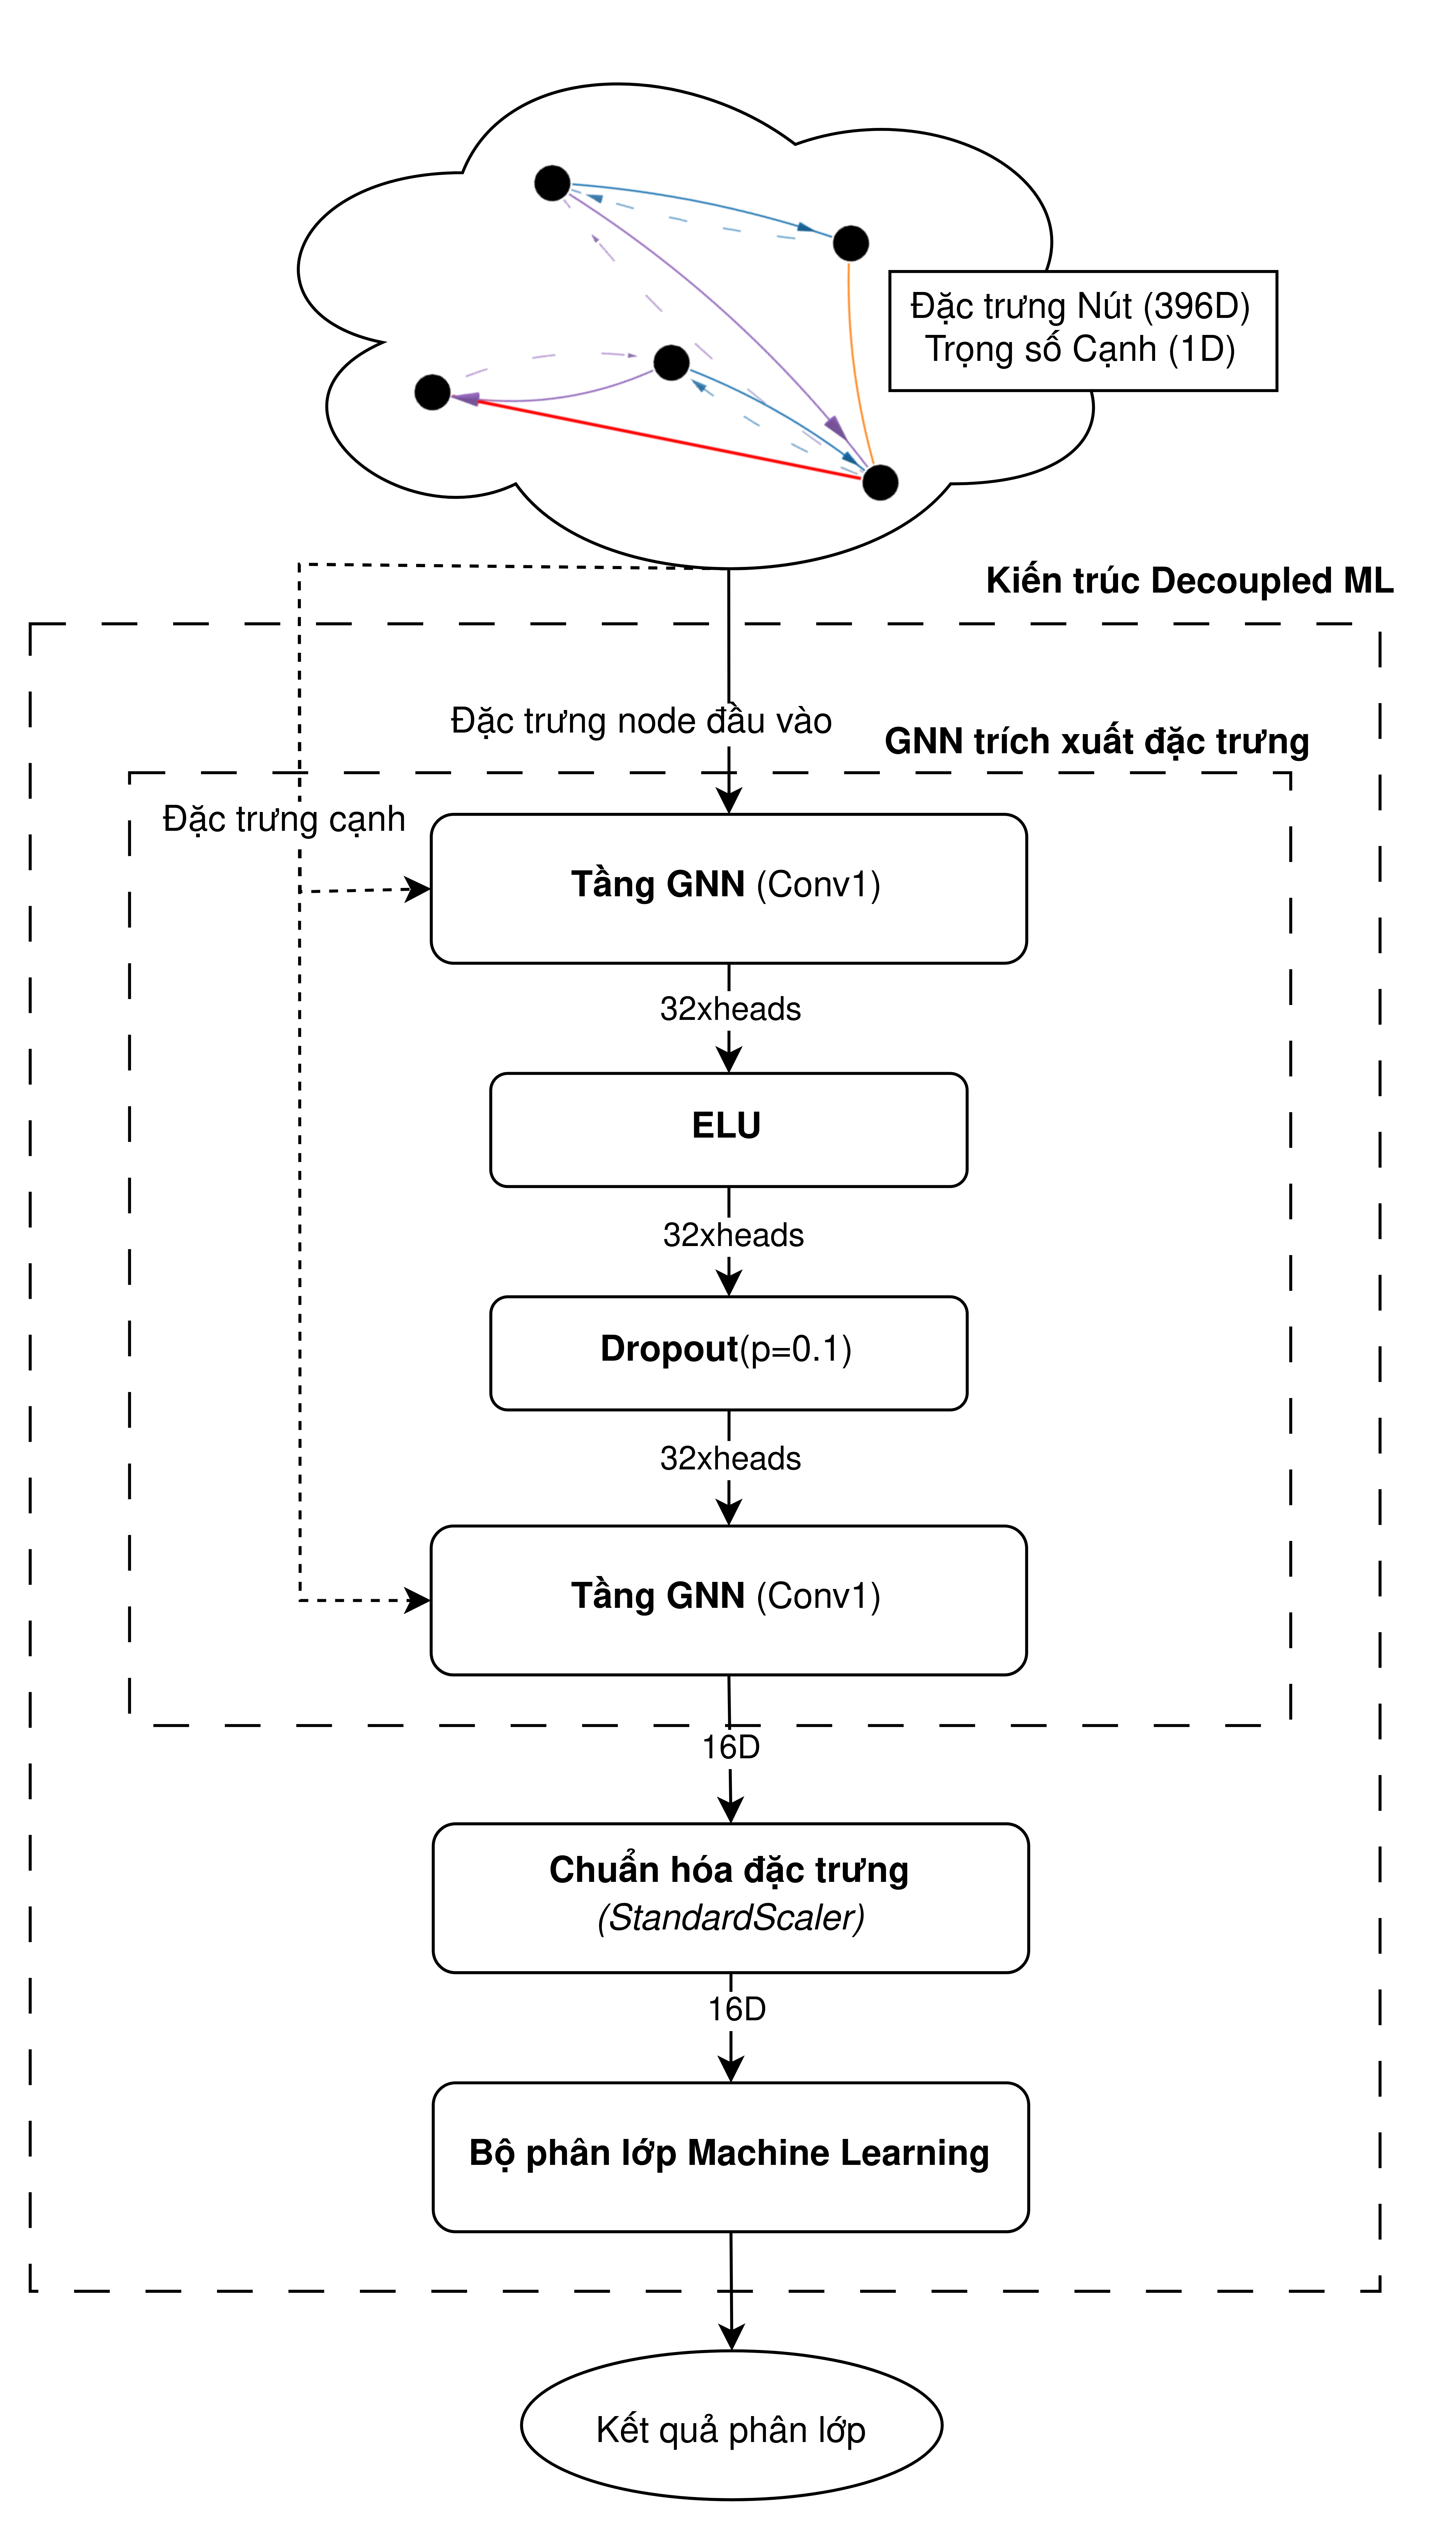
\includegraphics[width=0.65\linewidth]{images/part-02/chap-02/sec-01/DecoupledMLArchitecture.png}
    \vspace{0.2cm}
    \caption{Sơ đồ luồng xử lý của kiến trúc Decoupled GNN-ML}
    \label{fig:DecoupledML}
\end{figure}

\textit{1.5.1. Cơ chế trích xuất đặc trưng và chuẩn hóa}\vspace{0.2cm}

\indent Để khắc phục tình trạng hiện tượng các mạng nơ-ron gặp khó khăn trong việc điều chỉnh biên độ đầu ra một cách chính xác do sai lệch về phạm vi dự đoán — nghiên cứu này tận dụng GNN như một bộ trích xuất biểu diễn cấu trúc:

\begin{itemize}[label={--}, itemsep=3pt]
    \item \textbf{Trích xuất đặc trưng:} Hệ thống thực hiện trích xuất vector từ tầng tích chập thứ hai. Việc này giúp thu thập các biểu diễn đã được tổng hợp thông tin liên kết láng giềng nhưng chưa bị áp đặt bởi các quy tắc quyết định.
    \item \textbf{Vector đặc trưng:} Kết quả là một vector $16$ chiều mang tính chất nén thông tin quan hệ trong đồ thị.
    \item \textbf{Chuẩn hóa đặc trưng:} Sử dụng \texttt{StandardScaler} để điều chỉnh quy mô các giá trị về phân phối chuẩn, tạo điều kiện cho bộ phân lớp máy học phía sau thiết lập các siêu phẳng phân tách hiệu quả hơn.
\end{itemize}

\textit{1.5.2. Bộ phân lớp dựa trên Machine Learning}\vspace{0.2cm}

Thay vì bắt mạng nơ-ron phải tự học các quy tắc phân ngưỡng phức tạp, nghiên cứu thực hiên đưa các vector biểu diễn đồ thị sang các thuật toán học máy truyền thống để xây dựng các ranh giới phân quyết rõ ràng. Các mô hình được thiết lập cấu hình chuyên biệt để xử lý vector nhúng $16$ chiều và phân tách $4$ cấp độ rủi ro:

\begin{itemize}[label={--}, itemsep=3pt]
    \item \textbf{K-Nearest Neighbors (KNN):} Thực hiện phân loại dựa trên mật độ phân phối với cấu hình $5$ láng giềng gần nhất ($k=5$). Đặc biệt, mô hình sử dụng cơ chế trọng số theo khoảng cách (\textit{distance weights}), giúp các láng giềng có độ tương đồng cao trong không gian nhúng có tầm ảnh hưởng lớn hơn đến kết quả dự đoán. Cách tiếp cận này giúp nhận diện chính xác các cụm tài khoản có cùng kịch bản hành vi dựa trên khoảng cách hình học thuần túy.
    
    \item \textbf{Linear SVC:} Thiết lập hệ thống siêu phẳng phân tách với giới hạn tối đa $3000$ vòng lặp để đảm bảo sự hội tụ trên không gian ẩn $16$ chiều. Để giải quyết tình trạng mất cân bằng dữ liệu giữa các lớp rủi ro, mô hình tích hợp tham số \texttt{class\_weight}, giúp điều chỉnh tầm quan trọng của các ít xuất hiện do dữ liệu nhãn mất cân bằng. Việc này cho phép SVC xây dựng các ranh giới phân tách hiệu quả hơn, đặc biệt là trong việc phân biệt giữa các lớp rủi ro có sự chồng lấn về đặc trưng.
    
    \item \textbf{Random Forest:} Sử dụng hệ thống tập hợp gồm $100$ cây quyết định độc lập kết hợp với chiến lược trọng số lớp (\textit{class weighting}). Mô hình thực hiện các phân tách đa tầng trên từng chiều đặc trưng của vector nhúng, thiết lập các điều kiện rẽ nhánh phức tạp để phân biệt rõ ràng giữa các cấp độ rủi ro.
    
    \item \textbf{XGBoost:} Triển khai thuật toán tăng cường gradient với mục tiêu tối ưu hóa xác suất đa lớp (\textit{multi:softprob}) cho $4$ nhãn mục tiêu. Thông qua việc học từ sai số và sử dụng hàm mất mát \textit{mlogloss}, mô hình tập trung tinh chỉnh các ranh giới tại "vùng xám" — nơi các thực thể tấn công tinh vi cố gắng mô phỏng đặc trưng của nhóm an toàn. Việc sử dụng trọng số mẫu (\textit{sample weights}) trong quá trình huấn luyện giúp XGBoost nâng cao khả năng phân loại các mức độ rủi ro.
\end{itemize}